\documentclass[../main.tex]{subfiles}

\begin{document}

\subsection{Sprints}

\tocless\subsubsection{Sprint uge 15 - 16}
\paragraph{Goal}\mbox{}\\
I dette sprint vil teamet være fokuseret på at få oprettet grundstrukturen for kodebasen ud fra den udarbejdede analysemodel.

\paragraph{Retrospektiv}\mbox{}\\
Det var ikke hensigtsmæssigt at lave detaljerede brugsmønstre for alle brugsmønstrene i produkt backloggen. Da man først brude have lavet detaljerede brugsmønstre når man starter arbejdet med dem. Teamet har fået praktisk erfaring med scrum og har fundet ud af at det er svært at pririotere tid. Der er også lavet en del grundarbejde i denne sprint som vil gøre det nemmere i de kommende sprint.

\begin{center}
\begin{figure}[H]
\footnotesize
\centering
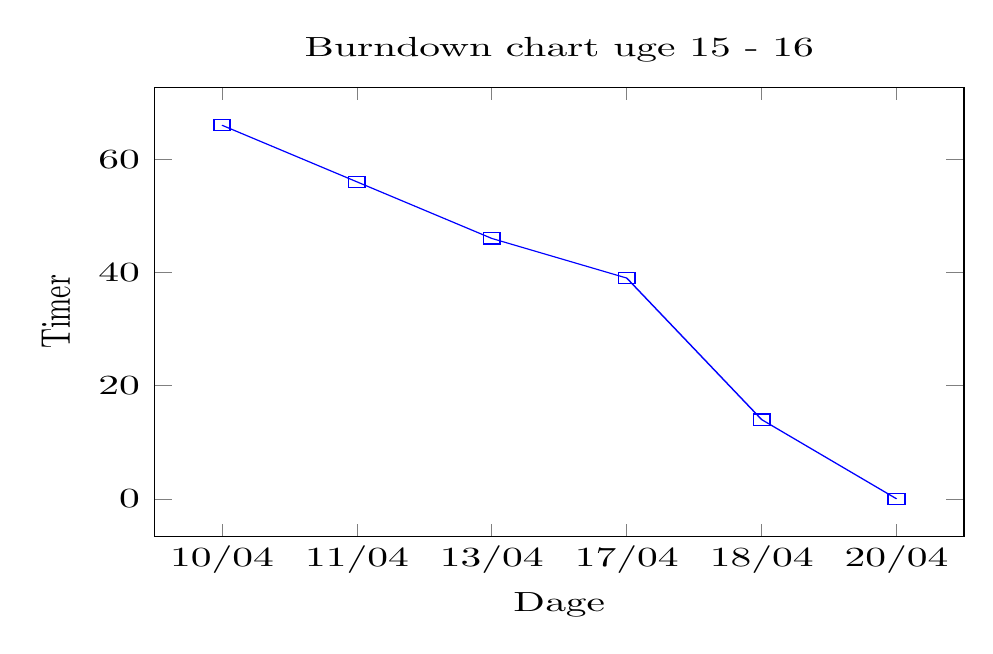
\begin{tikzpicture}[xscale=1.5]
\begin{axis}[
    title={Burndown chart uge 15 - 16},
    xlabel={Dage},
    ylabel={Timer},
    xtick={0, 1, 2, 3, 4, 5},
    xticklabels={$10/04$, $11/04$, $13/04$, $17/04$, $18/04$, $20/04$},
]
 
\addplot[
    color=blue,
    mark=square,
    ]
    coordinates {
    (0,66)(1,56)(2,46)(3,39)(4,14)(5,0)
    };
    %\legend{CuSO$_4\cdot$5H$_2$O}
 
\end{axis}
\end{tikzpicture}
    \caption{Burndown chart uge 15 - 16}
    \label{fig:burndown_15_16}
\end{figure}
\end{center}

\begin{center}
\begin{table}[H]
\resizebox{\textwidth}{!}{%
    \begin{tabular}{| l | c | c | c | c | c | c |} 
    \hline
    Opgaver								  							 & 10/04 & 11/04 & 13/04 & 17/04 & 18/04 & 20/04 \\ \hline
    Opsætning af 3-lags arkitektur									 & 4  & 4  & 4 & & & \\ \hline
    Analysemodel													 & 24 & 24 & 24 & 24 & & \\ \hline
    Basisklasse opsætning ud fra analysemodel						 & 18 & 18 & 18 & 15 & 14 & \\ \hline
    Detaljeret Brugsmønster											 & 10 & & & & & \\ \hline
    Kundemøde EG Team Online										 & 10 & 10 & & & & \\ \hline
    Total                                 							 & 66 & 56 & 46 & 39 & 14 & 0 \\ \hline
    \end{tabular}}
        \caption{Sprint backlog uge 15 - 16}
    \label{tab:sprint_backlog_15_16}
\end{table}
\end{center}

\tocless\subsubsection{Sprint uge 21 - 22}
\paragraph{Goal}\mbox{}\\
Teamets mål er at færdiggøre implementeringen i forhold til database og domain-laget, derudover skal alle manglende rapport afsnit skrives og den samlet rapport skal rettes og afleveres den. 31. Maj.

\begin{center}
\begin{figure}[H]
\footnotesize
\centering
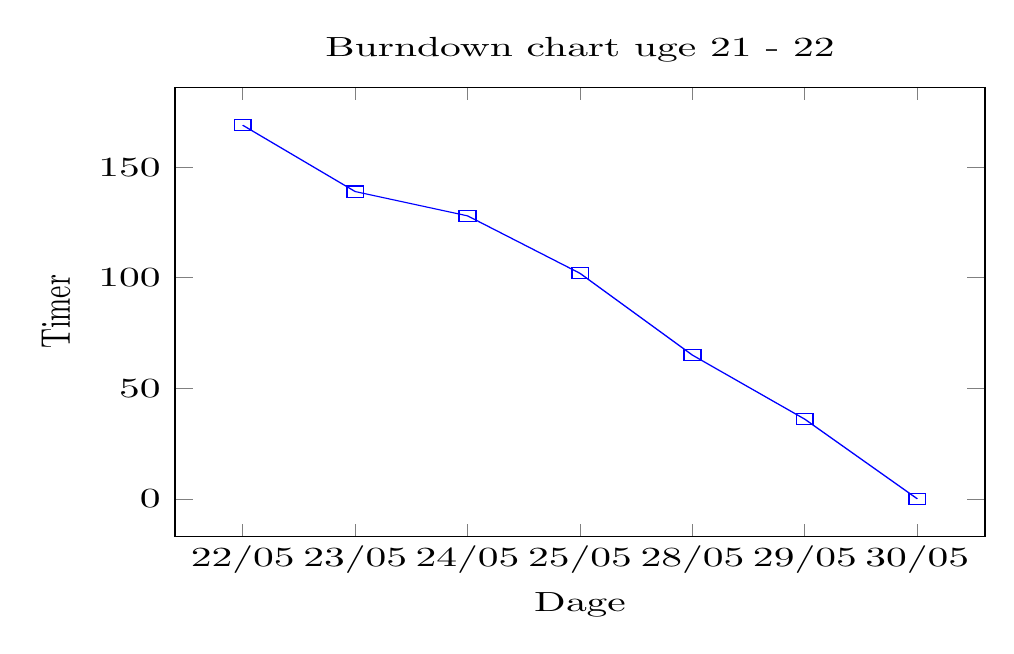
\begin{tikzpicture}[xscale=1.5]
\begin{axis}[
    title={Burndown chart uge 21 - 22},
    xlabel={Dage},
    ylabel={Timer},
    xtick={0, 1, 2, 3, 4, 5, 6},
    xticklabels={$22/05$, $23/05$, $24/05$, $25/05$, $28/05$, $29/05$, $30/05$},
]

\addplot[
    color=blue,
    mark=square,
    ]
    coordinates {
    (0,169)(1,139)(2,128)(3,102)(4,65)(5,36)(6,0)
    };
    %\legend{CuSO$_4\cdot$5H$_2$O}
 
\end{axis}
\end{tikzpicture}
    \caption{Burn down chart uge 21 - 22}
    \label{fig:burn_down_21_22}
\end{figure}
\end{center}


\begin{center}
\begin{table}[H]
\resizebox{\textwidth}{!}{%
    \begin{tabular}{| l | c | c | c | c | c | c | c |} 
    \hline
    Opgaver								  							 & 22/05 & 23/05 & 24/05 & 25/05 & 28/05 & 29/05 & 30/05 \\ \hline
    GDPR research													 & 2 & 1 &  & & & & \\ \hline
    Forbind Registrere at borgeren er informeret om rettigheder og pligter med DB   & 4 & 1 & & & & & \\ \hline
    Forbind Registrere basisoplysninger vedr. borger  med DB  		 & 4 & 1 &  &  &  & & \\ \hline
    Forbind Registrere eventuelle særlige forhold  med DB     		 & 2 &  &  &  &  & & \\ \hline
    Forbind Fastlægge det videre forløb   med DB 					 & 2 &  &  &  &  & & \\ \hline
    Forbind login med DB										     & 8 &  &  &  &  & & \\ \hline
    Rapport Omslag										             & 2 & 2 & 2 & 2 &  & & \\ \hline
    Resume/Abstract										             & 4 & 4 & 4 & 4 & 4 & 4 & \\ \hline
    Forord										                     & 2 & 2 & 2 & 2 & 1 & 1 & \\ \hline
    Læsevejledning									                 & 4 & 4 & 4 & 4 & 4 & 4 & \\ \hline
    Ordliste 	        											 & 2 & 2 & 2 & 2 & 1 & 1 & \\ \hline
    Redaktionel 	        									     & 5 & 5 & 5 & 5 & 5 & 3 & \\ \hline
    Indledning 	        											 & 6 & 1 &  &  1 &   &  & \\ \hline
    Metode og planlægning 	        								 & 8 & 2 & 1 & 1 &   &  & \\ \hline
    Elaboration: Krav specifikation 	        					 & 10 & 10 & 5 & 3 & 1 & 1 & \\ \hline
    Elaboration: Analyse 	        								 & 6 & 6 & 6 & 3 & 1 & 1 & \\ \hline
    Elaboration: Design: Arkitektur 	        				     & 4 & 4 & 4 & 2 & 1 & 1 & \\ \hline
    Elaboration: Design: Designmodel 	        				     & 10 & 10 & 9 & 5 & 2 & 1 & \\ \hline
    Elaboration: Design: Persitences 	        				     & 8 & 8 & 8 & 4 & 1 & 1 & \\ \hline
    Elaboration: Implementering: Arkitektur 	        		     & 8 & 8 & 8 & 1 &  & & \\ \hline
    Elaboration: Implementering: Persitences 	        		     & 8 & 8 & 8 & 3 & 2 & 1 & \\ \hline
    Elaboration: Implementering: Login 	        		     		 & 16 & 16 & 16 & 16 & 10 & 2 & \\ \hline
    Elaboration: Implementering: Sagsåbning 	        		     & 16 & 16 & 16 & 16 & 10 & 2 & \\ \hline
    Elaboration: Test												 & 6 & 6 & 6 & 6 & 3 & 1 & \\ \hline
    Elaboration: Konklusion										 	 & 4 & 4 & 4 & 4 & 4 & 1 & \\ \hline
    Evaluering										 	 		 	 & 6 & 6 & 6 & 6 & 5 & 3 & \\ \hline
    Konklusion														 & 8 & 8 & 8 & 8 & 8 & 6 & \\ \hline
    Referenceliste													 & 4 & 4 & 4 & 4 & 2 & 2 & \\ \hline
    Total                                 							 & 169 & 139 & 128 & 102 & 65 & 36 & 0 \\ \hline
    \end{tabular}}
    \caption{Sprint backlog uge 21 - 22}
    \label{tab:sprint_backlog_21_22}
\end{table}
\end{center}

\end{document}